
%(BEGIN_QUESTION)
% Copyright 2012, Tony R. Kuphaldt, released under the Creative Commons Attribution License (v 1.0)
% This means you may do almost anything with this work of mine, so long as you give me proper credit

The following ammonium nitrate production process was shut down for an extended period of time (typically, this kind of event is called an ``outage'' or a ``turnaround'') to perform maintenance on components that could not be worked on while the unit was running:

$$\includegraphics[width=15.5cm]{i0008rx01.eps}$$

Unfortunately, the purchasing agent for the company mistakenly ordered the wrong type of valve trim on all the control valves being rebuilt.  Instead of ordering equal-percentage trim for each of the valves as originally specified, the purchaser accidently ordered {\it linear} trim.  

When the work was completed and the unit re-started, operations personnel began to notice the scrubber level control loop behaving poorly: the scrubber liquid level would not remain stable at setpoint the way it used to before the outage.  

An instrument technician sent to diagnose this problem noticed that valve LV-35 was sporting a fresh coat of paint, suggesting it had been rebuilt during the outage, and following this clue the technician was able to discover the trim misconfiguration as being the cause of the instability.

After fixing this problem, the same technician decided to investigate other control valves in the unit that had been rebuilt.  FV-25 was another one of the valves that had the wrong characterization of trim installed, and yet the rundown tank level control system was not misbehaving: LIC-26 was able to maintain liquid level at setpoint regardless of load changes or setpoint changes.

\vskip 10pt

Explain why a change of valve trim characteristic caused problems for the scrubber's level control system, but not for the rundown tank's level control system.

\vskip 20pt \vbox{\hrule \hbox{\strut \vrule{} {\bf Suggestions for Socratic discussion} \vrule} \hrule}

\begin{itemize}
\item{} Will an incorrect trim characterization in FV-25 have any deleterious effects at all?
\end{itemize}

\underbar{file i01694}
%(END_QUESTION)





%(BEGIN_ANSWER)

Hint: the rundown tank's level control system is {\it cascaded} to a flow controller (FIC-25).

%(END_ANSWER)





%(BEGIN_NOTES)

The cascaded level/flow system of LIC-26/FIC-25 ``shields'' the level controller from any control valve problems, since the flow controller handles those problems before they become severe enough to affect level.  This does not mean, however, that the characterization of FV-25 is irrelevant -- FIC-25 will experience instability as a result of the wrong trim being installed.  Instabilty in the fast-acting flow control loop, however, may not reveal itself in the slower-acting rundown tank level control loop.








\filbreak \vskip 20pt \vbox{\hrule \hbox{\strut \vrule{} {\bf Virtual Troubleshooting} \vrule} \hrule}

\noindent
{\bf Predicting the effect of a given fault:} present each of the following faults to the students, one at a time, having them comment on all the effects each fault would produce.

\begin{itemize}
\item{} Rundown tank level controller tuned with too-aggressive integral action
\item{} Excessive stiction in FV-25
\item{} FT-25 failed with low (0\%) signal
\item{} LT-26 failed with high (100\%) signal
\item{} Restrictor in FV-25 positioner plugs (assume air-to-open valve)
\end{itemize}


\vskip 10pt


\noindent
{\bf Identifying possible/impossible faults:} present symptoms to the students and then have them determine whether or not a series of suggested faults could account for all the symptoms, explaining {\it why} or {\it why not} for each proposed fault:

\begin{itemize}
\item{} Symptom: {\it }
\item{} 
\item{} 
\item{} 
\end{itemize}


\vskip 10pt


\noindent
{\bf Determining the utility of given diagnostic tests:} present symptoms to the students and then propose the following diagnostic tests one by one.  Students rate the value of each test, determining whether or not it would give useful information (i.e. tell us something we don't already know).  Students determine what different results for each test would indicate about the fault, if anything:

\begin{itemize}
\item{} Symptom: {\it }
\item{}  -- {\bf Yes/No}
\item{}  -- {\bf Yes/No}
\end{itemize}


\vskip 10pt


\noindent
{\bf Diagnosing a fault based on given symptoms:} imagine the ??? fails ??? in this system (don't reveal the fault to students!).  Present the operator's observation(s) to the students, have them consider possible faults and diagnostic strategies, and then tell them the results of tests they propose based on the following symptoms, until they have properly identified the nature and location of the fault:

\begin{itemize}
\item{} {\it }
\item{} 
\item{} 
\end{itemize}
%INDEX% Control, strategies: cascade
%INDEX% Process: ammonium nitrate production (realistic P&ID shown)

%(END_NOTES)


